\documentclass[]{IEEEtran}

\usepackage[utf8]{inputenc}
\usepackage{float, graphicx, booktabs, siunitx}
\usepackage{microtype, amsmath}

\usepackage{inconsolata}
\usepackage[italian]{babel}

\newcommand{\code}[1]{\texttt{\small #1}}

\title{Modellazione in SystemC di un cifrario basato su algoritmo XTEA con possibili utilizzi}
\author{Massimiliano Incudini - VR433300}

\begin{document}
\maketitle

\begin{abstract}
    Il seguente documento documenta il lavoro svolto durante il la prima parte del modulo di laboratorio del corso Progettazione di Sistemi Embedded (aa 2018/2019). Il suo obiettivo è illustrare le scelte progettuali effettuate per ognuna delle diverse versioni del cifratore XTEA.
\end{abstract}

\section{Introduzione}

Il progetto consiste nello sviluppare un cifrario il cui funzionamento è basato sull'algoritmo eXtended TEA fornito insieme alla consegna. Il cifrario dovrà essere implementato come modulo (insieme al proprio testbench) nelle versioni:
\begin{itemize}
    \item RTL: il modulo viene diviso in due processi, uno che ne rappresenta la propria FSM e l'altro che ne rappresenta il datapath;
    \item TLM untimed: il modulo viene implementato attraverso le classi di TLM senza tenere traccia dell'informazione temporale della simulazione;
    \item TLM loosely timed: il modulo è simile al precedente, con la differenza che tiene parzialmente conto dell'informazione temporale ed utilizza la tecnica del temporal decoupling per ottimizzare le prestazioni della simulazione;
    \item TLM approximatively timed 4-phases: il modulo è progettato per essere interrogato attraverso chiamate TLM non bloccanti, ogni transazione attraversa quattro fasi che richiedono sincronizzazione esplicita.
\end{itemize}

Viene inoltre richiesto di implementare un sistema formato da un controllore, una valvola ed un serbatoio d'acqua. Il controllore riceve il livello dell'acqua dal serbatoio, e manda alla valvola il comando per aprire e chiudere il rubinetto di conseguenza. Il sistema dovrà essere sviluppato in SystemC-AMS.

Infine viene richiesto di modificare il sistema precedente implementando il controllore con TLM ed assicurandosi che mandi le transazioni criptate con XTEA, aggiungengo transattori ai moduli AMS e ponendo tra il controllore e la valvola un decifratore XTEA in RTL (con proprio transattore).



\section{Modellazione RTL}

La prima versione del cifratore (RTL) viene implementata a partire dal sorgente fornito. Il primo compito svolto è stato schematizzare il codice in un diagramma di flusso (Figura~\ref{fig:algo}). 

\begin{figure*}[htbp]
    \centering
    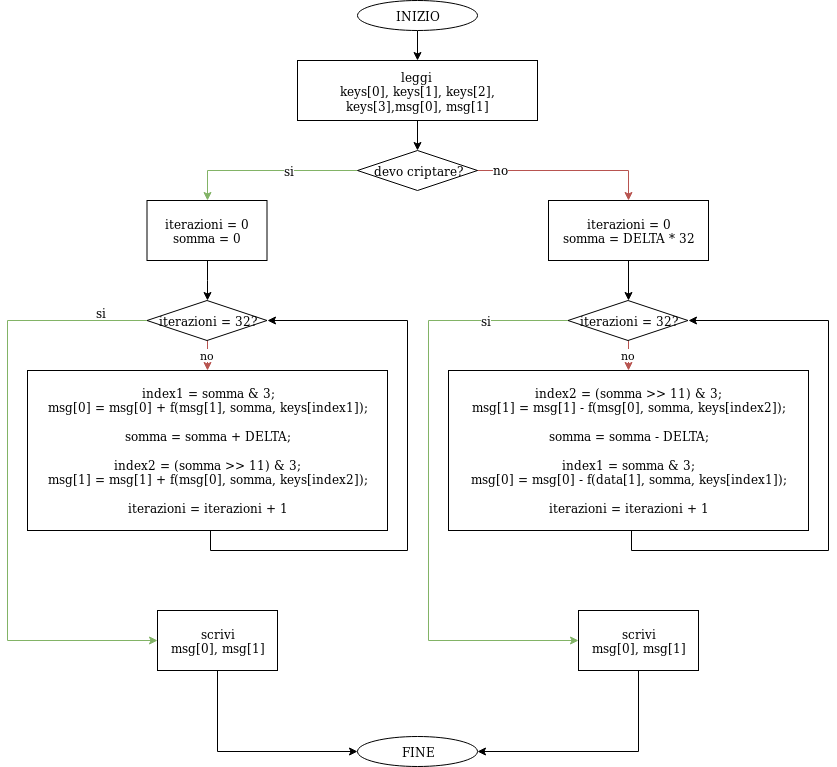
\includegraphics[width=0.7\textwidth]{schemi/algo.png}
    \caption{Algoritmo ad alto livello del cifratore. NB: La funzione $f(a,b,c)$ è un'espressione che corrisponde a $(((a \ll 4) \oplus (a \gg 5)) + a) \oplus (b + c)$.}
    \label{fig:algo}
\end{figure*}

Questo permette di estrarre gli input e gli output che servono al modulo per funzionare. Una prima soluzione potrebbe essere prende in input tutti i dati che servono in una volta sola: la chiave, i dati da elaborare, la modalità di esecuzione.

In realtà l'interfaccia risulta grossolana: il cifratore probabilmente dovrà elaborare un discreto numero di dati utilizzando sempre la stessa chiave (intesa come il gruppo di 128 bit). Risulta inutile passarla sempre quando per la maggior parte delle computazioni questa rimarrà identica. Si sceglie quindi di togliere l'input relativo alla chiave. Questa verrà passata all'inizio della computazione utilizzando la porta \code{data}. Poiché la porta \code{data} è di 64bit e la chiave è grande il doppio, occorrerà passarla in due volte. Otteniamo lo schema che segue:
\begin{center}
    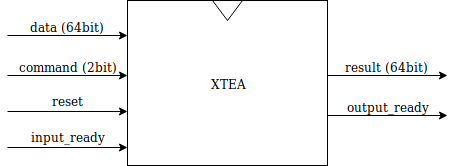
\includegraphics[width=0.35\textwidth]{schemi/rtl_interface.png}
\end{center}

Le porte hanno il seguente significato:
\begin{itemize}
    \item \code{clock} (in input);
    \item \code{reset} (in input): quando attivo alto, riporta il modulo allo stato iniziale;
    \item \code{command} (in input, 2bit): comando da eseguire sul modulo;
    \item \code{data} (in input, 64bit): valore da processare;
    \item \code{input\_ready} (in input): quando attivo alto, si possono leggere i dati in input;
    \item \code{result} (in output, 64bit): risultato della computazione;
    \item \code{output\_ready} (in output): quando è attivo alto, la computazione è terminata;
\end{itemize}

L'azione corrispondente ai valori forniti in input è presente in Tabella~\ref{tab:azioni}. Una volta che il modulo ha finito la computazione, viene attivato il segnale \code{output\_ready} e viene mantenuto attivo un solo ciclo di clock. Durante questo periodo di tempo si può leggere il valore della porta \code{result}.

\begin{table*}[htbp]
    \centering
    \begin{tabular}{lllp{5cm}}
        \toprule
        reset & input\_ready & command & azione \\ \cmidrule{1-4}
         \code{1} & \code{-} & \code{--} &	riporta il sistema allo stato iniziale
        \\ \code{0} & \code{0} & \code{--} &	non fare nulla
        \\ \code{0} & \code{1} & \code{00} &	memorizza il valore su data all’interno del sistema come i primi 64bit della chiave
        \\ \code{0} & \code{1} & \code{01} &	memorizza il valore su data all’interno del sistema come i secondi 64bit della chiave
        \\ \code{0} & \code{1} & \code{10} &	avvia la criptazione, il messaggio è il valore su data
        \\ \code{0} & \code{1} & \code{11} &	avvia la decriptazione, il messaggio è il valore su data \\ \bottomrule
    \end{tabular}
    \caption{Tabella delle azioni}
    \label{tab:azioni}
\end{table*}

Si è deciso di dividere il modulo in due funzioni separate: una funzione è \code{fsm} e l'altra \code{datapath}. La prima ha il compito di leggere i dati in input e memorizzarli all'interno del modulo, scandire l'avanzamento della computazione modificando la variabile di stato, e scrivere i valori in output. La seconda si occupa di elaborare espressioni aritmetiche anche semplici. 

Si può notare nell'algoritmo in Figura~\ref{fig:algo} che buona parte dei due blocchi più grandi, quelli contenenti i calcoli, si sovrappone. Per questo il modulo cercherà di sfruttare quando può questa sovrapposizione per minimizzare l'area (del datapath, nella quale vengono effettuate queste computazioni). 

Inoltre le operazioni $\text{index} = x \text{\&} 3, \; \text{index} = (x \gg 11) \text{\&} 3$ usate per calcolare quale parte di chiave si traducono in una semplice estrazione di bit dall'operando, quindi non serve passare dal datapath.

Il compito della FSM è legge gli input e li salva all'interno delle propri registri, gestisce lo stato, comunica col datapath e scrive gli output. Il datapath legge i dati dai registri della FSM e li sposta nei propri registri effettua le operazioni aritmetiche. In Figura~\ref{fig:internal} puoi vedere la mappa dei registri. Ogni registro è scritto o solo dalla FSM o solo dal datapath.

\begin{figure}[htbp]
    \centering
    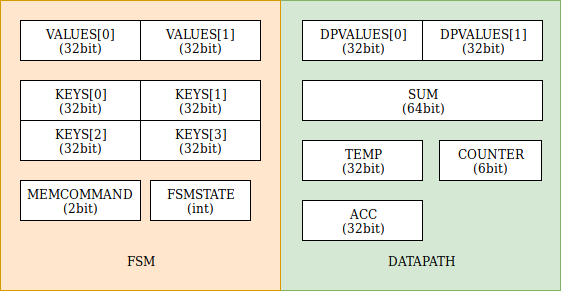
\includegraphics[width=0.45\textwidth]{schemi/rtl_registers.png}
    \caption{Registri interni al modulo}
    \label{fig:internal}
\end{figure}

Lo schema compatto di FSM e datapath è presente sottoforma di schema in Figura~\ref{fig:efsm}. I cerchi sono gli stati, le etichette sulle freccie indicano la condizione con la quale viene cambiato lo stato. In rettangoli verdi sono i calcoli svolti dal datapath. Come si può notare, le operazioni fatte in alcuni stati sono uguali, il che ci permette di ottimizzare per area il nostro modulo. 

\begin{figure*}[htbp]
    \centering
    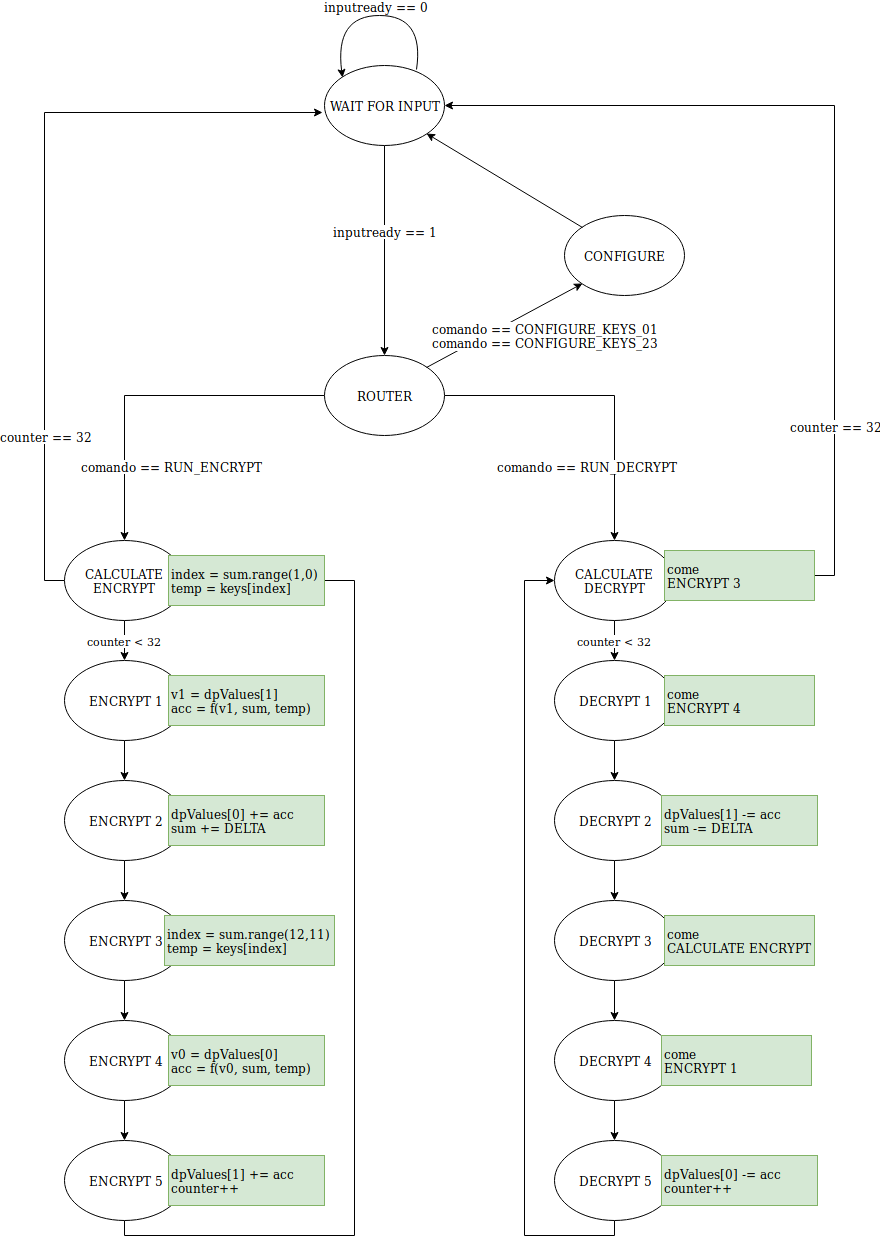
\includegraphics[width=0.7\textwidth]{schemi/rtl_efsm.png}
    \caption{Diagramma degli stati. Le transazioni sono comandate dalla FSM. In verde sono presenti le elaborazioni fatte dal datapath}
    \label{fig:efsm}
\end{figure*}
\newpage
\section{Modellazione TLM}

Le successive versioni del cifratore sono modellate usando il TLM. Il framework è stato sviluppato al di sopra di SystemC, ogni modulo TLM è un modulo di SystemC che eredita anche ulteriori interfacce. Il modulo XTEA (target) implementa anche l'interfaccia \code{ tlm::tlm\_fw\_transport\_if<>} (forward) mentre il suo testbench implementa l'interfaccia \code{ tlm::tlm\_bw\_transport\_if<>} (backward). I due moduli comunicano attraverso porte dette dette socket. Le interfacce forward devono avere al loro interno almeno una socket \emph{target} (per ricevere transazioni) e quelle backward devono avere almeno una socket \emph{initiator} (per iniziare transazioni). 

Le transazioni si scambiano sempre una struttura \code{ tlm::tlm\_generic\_payload} che al suo interno contiene un puntatore ad un oggetto definito dall'utilizzatore, che rappresenta il dato da scambiare durante la transazione. Nel nostro caso questo oggetto è un'istanza di \code{ struct Packet}. Essa ha al suo interno il comando per il target ed l'operando su cui lavorare. 

\subsection{Modellazione TLM Untimed}

Il comportamento del target è codificato nella funzione \code{b\_transport} che prende in input il \code{ tlm\_generic\_payload} ed una variabile che rappresenta il tempo. La chiamata, che verrà effettuata dall'initiator, è bloccante.

Il payload può essere di lettura o scrittura. Nel nostro caso è sempre sia di scrittura (il target esegue l'operazione) che di lettura (il target ritorna l'eventuale risultato). 

In questo caso l'informazione temporale non viene aggiornata. 

\subsection{Modellazione TLM Loosely Timed}

Questa versione differisce dalla precedente perchè viene parzialmente introdotta la gestione dell'informazione temporale. Il target nella funzione \code{ b\_transport} aggiornerà il tempo di esecuzione sommando il tempo, reale o presunto, dell'operazione richiesta dalla transazione. Si è a conoscenza del tempo reale solamente se si è già implementato il modulo a livello RTL. Nel nostro caso, possiamo settare il tempo pari a 798 cicli di clock. Il tempo di un ciclo di clock è richiesto come parametro del costruttore del target. 

La simulazione perfettamente sincronizzata dei componenti è costosa. Essa può essere velocizzata attraverso il \emph{temporal decoupling}. I processi possono essere eseguiti oltre il tempo della simulazione (non cedendo quindi il controllo allo scheduler) per un tempo massimo fissato detto \emph{quanto di tempo} o fino a che non è richiesta una sincronizzazione esplicita. Il guadagno di tempo si ottiene quindi riducendo il numero di context-switching. L'oggetto che mantiene la sincronia è detto \emph{quantum keeper}. Il metodo \code{sync} del quantum keeper cede il controllo allo scheduler. 

Il testbench conterrà quindi un oggetto della classe \code{ tlm\_utils::tlm\_quantumkeeper} che ne gestisce la sincronizzazione.

\subsection{Modellazione TLM Approximatively Timed (4 phases)}

La transazione è implementata tramite una sequenza di chiamate non bloccanti \code{nb\_transport\_[fw|bw]}, ognuna delle quali è una certa \emph{fase} della transazione. Solitamente le fasi sono quattro: \code{BEGIN\_REQ}, \code{END\_REQ}, \code{BEGIN\_RESP}, \code{END\_RESP}. Si possono comunque mettere un numero arbitrario di fasi, fino a rendere la simulazione anche precisa fino al clock. 

L'initiator chiama la forward con fase \code{BEGIN\_REQ}, e il target termina la transazione con fase \code{END\_REQ}, nel frattempo inizia a fare i calcoli per completare l'operazione richiesta. Una volta completata, il target chiama la backward con fase \code{BEGIN\_RESP} e i dati richiesti, ed l'initiator chiude la transazione con fase \code{END\_RESP}.

\subsection{Confronto delle prestazioni}

Procediamo a fare un confronto delle prestazioni delle quattro implementazioni. Ogni volta le chiavi vengono inizializzate una volta sola, poi vengono criptate e decriptate un milione di word generate casualmente. I risultati sono visibili in Tabella~\ref{tab:prestazioni}.

\begin{table}[htbp]
    \centering
    \begin{tabular}{lS[table-format=1.3,table-space-text-post = \si{\second}]S[table-format=1.3,table-space-text-post = \si{\second}]S[table-format=1.3,table-space-text-post = \si{\second}]S[table-format=3.3,table-space-text-post = \si{\second}]}
        \toprule
        & {UT} & {LT} & {AT4} & {RTL} \\\cmidrule{1-5}
        Real time   & 1.149\si{\second} & 1.757\si{\second} & 1.672\si{\second} & 174.062\si{\second} \\
        User time   & 1.144\si{\second} & 1.752\si{\second} & 1.672\si{\second} & 174.062\si{\second} \\
        System time & 0.004\si{\second} & 0.004\si{\second} & 0.000\si{\second} & 0.004\si{\second} \\\bottomrule
    \end{tabular}
    \caption{Confronto delle prestazioni}
    \label{tab:prestazioni}
\end{table}

Possiamo concludere che le prestazioni peggiori si ottengono con il modello RTL che è il più preciso. I tempi sono misurati con l'utility \code{time}.
\newpage
\section{Modellazione AMS}

Il sistema è composto da una tanica d'acqua, dalla valvola che regola l'apertura della tanica e dal proprio controllore.

\begin{figure}[htbp]
    \centering
    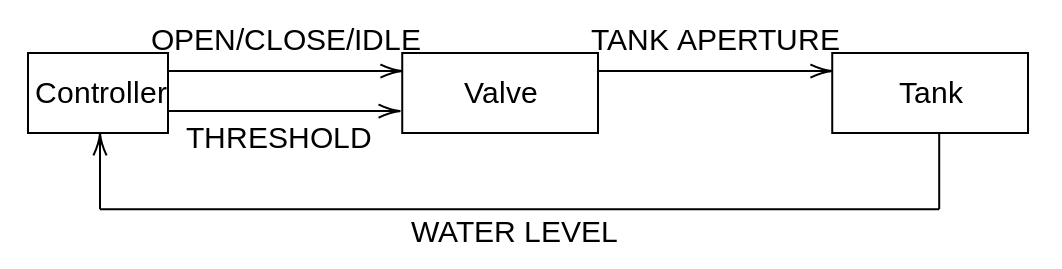
\includegraphics[width=0.5\textwidth]{schemi/ams-tank-valve.png}
    \caption{Schema del sistema tanica d'acqua}
    \label{fig:ams-tank-valve}
\end{figure}

La tanica mantiene al suo interno l'acqua. Il livello di riempimento è dato dalla funzione $x(t)$. Occorre che $5.0 \le x(t) \le 8.8$. Il livello di riempimento è dato dal sistema
\[ \begin{cases}
    \dot{x} = 0.6 a - 0.03 x \\
    x(0) = 0 
\end{cases} \]

La valvola aggiorna il livello proprio livello di apertura $a$ a seconda del comando che riceve dal controllore. I valori esatti sono presenti in Tabella~\ref{tab:ams-comandi}. In ogni caso occorre che $0 \le a(t) \le T$ con $T$ threshold in input dal controllore. Il valore iniziale si suppone sia $a(0) = 0$.

Il controllore monitore il livello dell'acqua e comanda la valvola di conseguenza. I comandi generati sono \code{OPEN}, \code{IDLE} e \code{CLOSE}. Un threshold (inteso come valore massimo) viene aggiornato secondo i valori di Tabella~\ref{tab:ams-comandi} e mandato alla valvola. Il suo valore iniziale è $T(0) = 0.7$.

\begin{table}[htbp]
    \centering
        \begin{tabular}{lrrrr}
        Segnale & Min lev & Max lev & Molt. threshold & Molt. $a$ \\ \hline
        \code{OPEN} & 0.0 & 5.0       & 1.1x &  0.25x \\
        \code{IDLE} & 5.0 & 8.8       & 1.0x &  0.00x \\
        \code{CLOSE} & 8.8 & $\infty$ & 0.7x & -0.25x
    \end{tabular}
    \caption{Comandi dati dal controllore alla valvola, range di livello di acqua del comando, moltiplicatore per l'aggiornamento del threshold, moltiplicatore per l'aggiornamento del livello di apertura}
    \label{tab:ams-comandi}
\end{table}

\subsection{Valvola}

La valvola è implementata tramite il modello discreto non conservativo AMS-TDF. Il suo compito è aggiornare il valore dell'apertura a seconda del comando ricevuto. La classe è definita tramite la macro \code{SCA\_TDF\_MODULE} e tutta la logica del componente è racchiusa nel metodo \code{processing}.

\subsection{Controllore}

Il controllore è implementato tramite il modello discreto non conservativo AMS-TDF. Il suo compito è ricevere il livello dell'acqua dal serbatoio e generare i comandi ed il threshold da passare alla valvola. a classe è definita tramite la macro \code{SCA\_TDF\_MODULE} e tutta la logica del componente è racchiusa nel metodo \code{processing}. Viene settato un ritardo obbligatorio sulla porta in input per poter definire un ordine di esecuzione per i componenti (scheduling). Il ritardo viene settato nel metodo \code{set\_attributes}. 

\subsection{Serbatoio}

Il serbatoio è implementato tramite AMS-LSF (a tempo continuo, non conservativo). 
\begin{figure}[htbp]
    \centering
    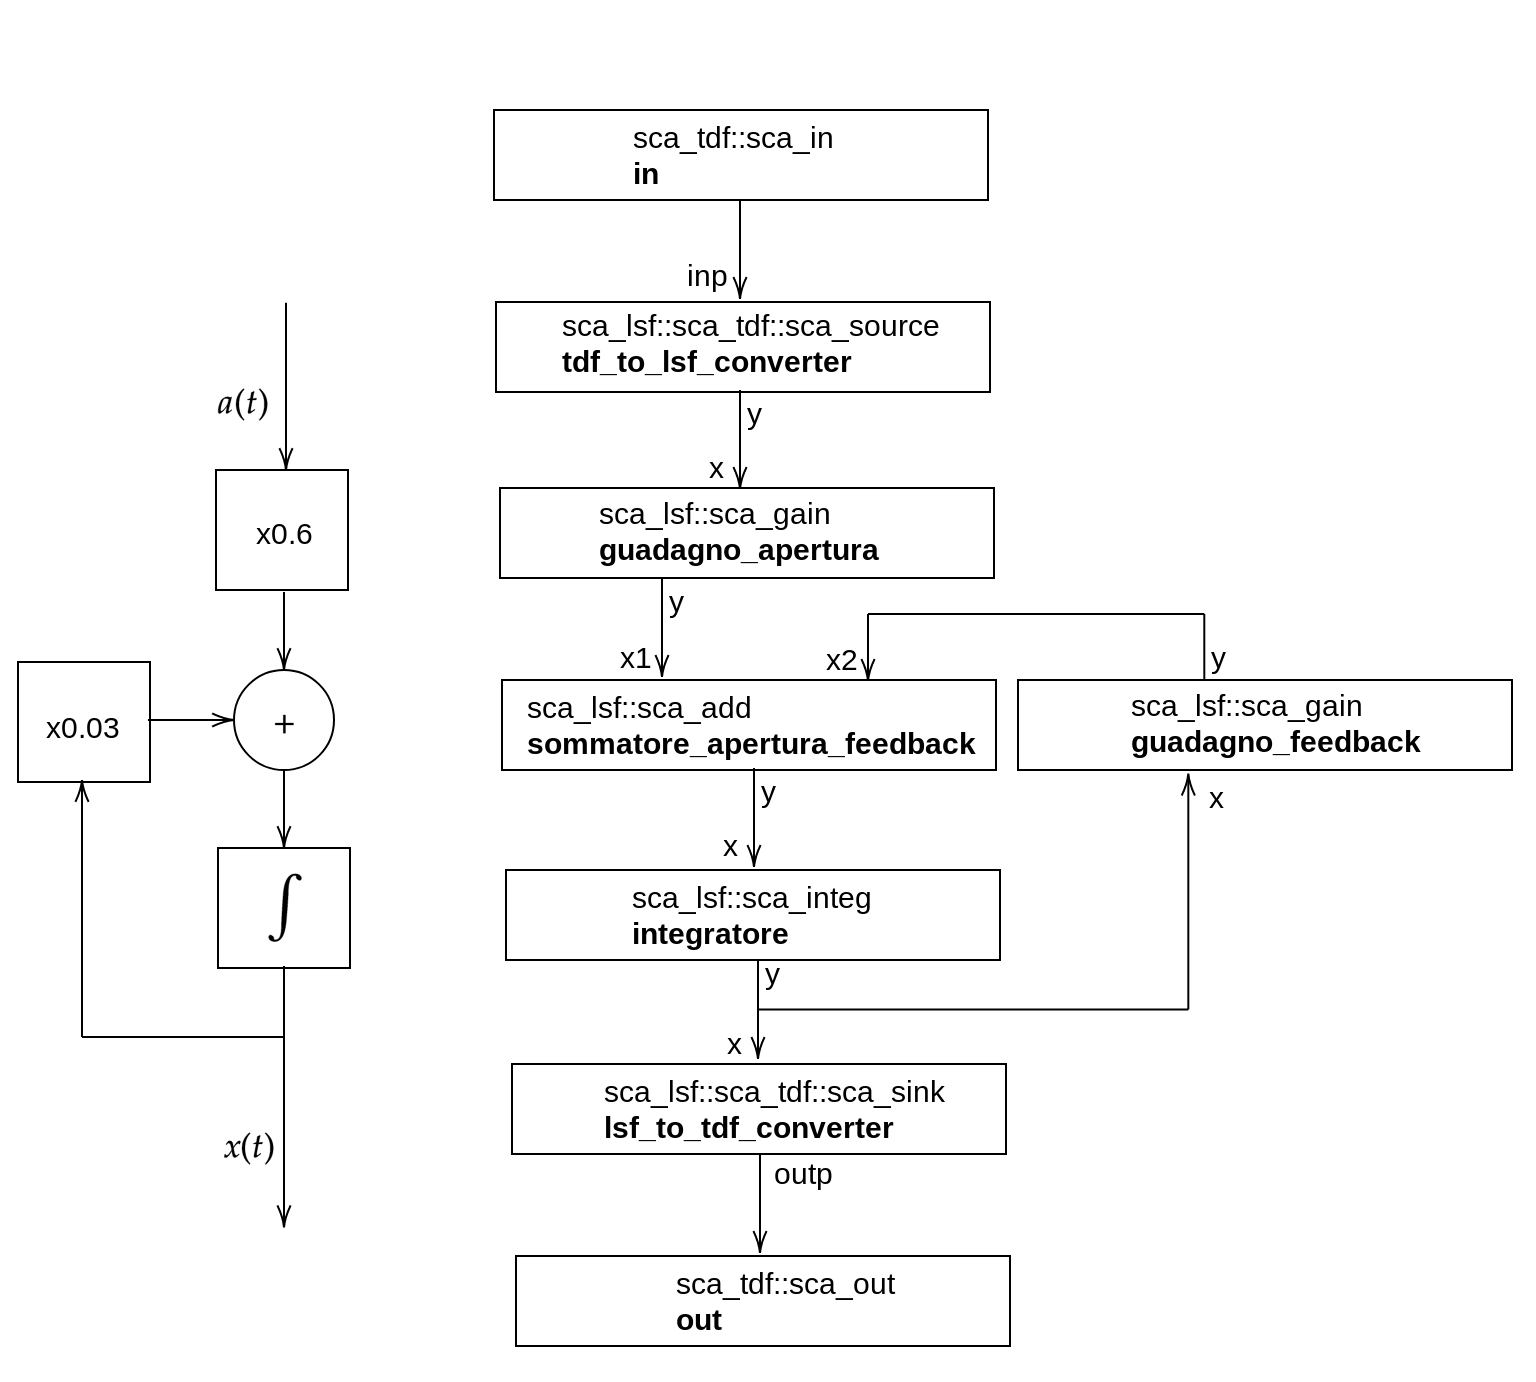
\includegraphics[width=0.5\textwidth]{schemi/ams-water-tank.png}
    \caption{Serbatoio. A sinistra lo schema ad alto livello, a destra lo schema con i componenti LSF. Per ogni blocco, la prima riga nel rettangolo è il tipo del componente, la seconda riga il nome, le etichette vicino alle frecce i nomi delle porte del componente.}
    \label{fig:ams-tank}
\end{figure}
Poichè il resto del sistema è a tempo discreto abbiamo due elementi che convertono il segnale TDF in LSF continuo e viceversa. I componenti utilizzati sono visibili in Figura~\ref{fig:ams-tank}.

\subsection{Risultato}

Vediamo di seguito che dopo diverse oscillazioni il livello dell'acqua si stabilizza ad $8.507$.
\begin{center}
    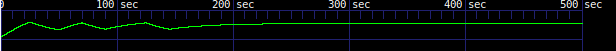
\includegraphics[width=0.5\textwidth]{schemi/ams-esito.png}
\end{center}
\newpage
\section{Modellazione Heterogeneous Platform}

La piattaforma eterogenea contiene componenti scritti con diversi formalismi e connessi tutti insieme. Essi sono:
\begin{itemize}
    \item controller, non più implementato con AMS ma come TLM (scelto modello untimed per semplicità;
    \item valvola, in AMS-TDF;
    \item serbatoio, in AMS-LSF internamente e AMS-TDF come interfaccia esterna;
    \item decrifratore XTEA, implementato in RTL.
\end{itemize}
Sono necessari ulteriori componenti "collante":
\begin{itemize}
    \item transattore che permette al sistema valvola-serbatoio di interfacciarsi con l'esterno tramite TLM;
    \item interfaccia RTL alla valvola, obbligatoria perchè TLM non riesce a comunicare direttamente con AMS;
    \item interfaccia RTL al serbatoio;
    \item transattore che collega controller, decifratore e sistema valvola-serbatoio; esso passa le richieste del controllore al resto del sistema, eventualmente decriptate.
\end{itemize}

\begin{figure}[htbp]
    \centering
    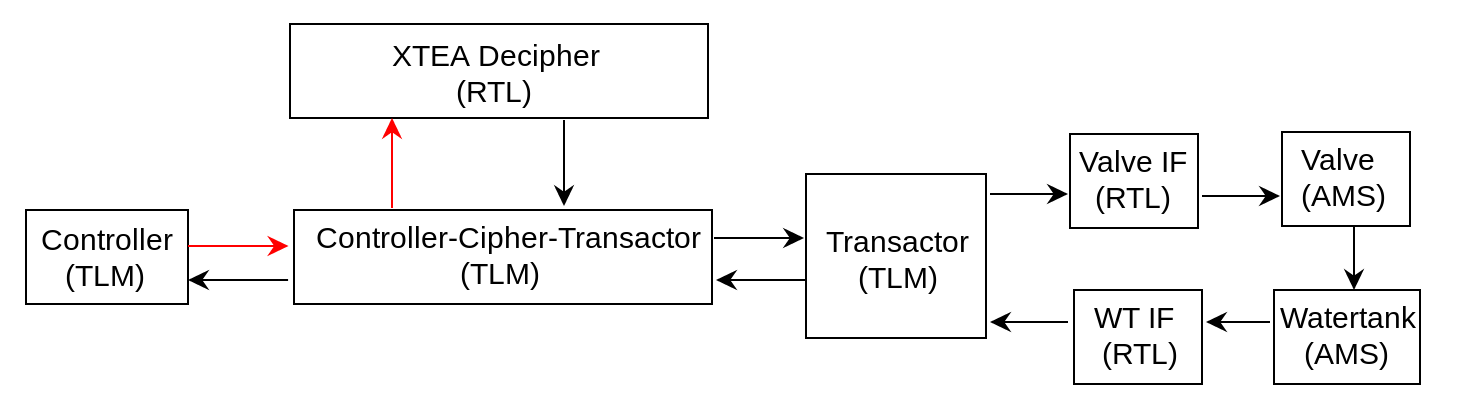
\includegraphics[width=0.5\textwidth]{schemi/het-schema.png}
    \caption{Schema della piattaforma eterogenea. Le freccie in rosso rappresentano il flusso di dati criptato.}
    \label{fig:heterog-platform}
\end{figure}

Lo schema del sistema può essere visto in Figura~\ref{fig:heterog-platform}. Ci sono due flussi di transazioni:
\begin{itemize}
    \item da \code{controller} al \code{controller-cipher-transactor};
    \item da \code{controller-cipher-transactor} a \code{transactor}.
\end{itemize}
Nel primo caso l'initiator è \code{controller}. Se la transazione è in scrittura allora questa conterrà i valori di threshold ed il comando per la valvola. I valori saranno criptati. Il target interroga il decifratore, ed una volta finita l'operazione crea una nuova transazione (secondo flusso). Non vengono ritornati valori all'initiator eccetto l'esito. Se la transazione è in lettura il target porterà avanti la richiesta con una transazione del secondo flusso. Il risultato viene ritornato all'initiator. In questo caso il decifratore non viene usato.

Nel secondo caso l'initiator è \code{controller-cipher -transactor} ed il target è il sistema valvola-serbatoio. Se la transazione è in scrittura allora passo i dati del payload alla valvola, altrimenti leggo i dati del serbatoio. 

\end{document}